\documentclass[tikz,border=10pt]{standalone}
% Shared look for every TikZ diagram. Load with % Shared look for every TikZ diagram. Load with % Shared look for every TikZ diagram. Load with \input{../../tools/tikz-style.tex}
\usepackage[T1]{fontenc}
\usepackage{lmodern}
\renewcommand{\sfdefault}{lmr}  % diagrams use the same serif as the text
\usetikzlibrary{arrows.meta, positioning, shapes.geometric, calc, fit, backgrounds}
\definecolor{cblue}{HTML}{4C78A8}
\definecolor{corange}{HTML}{F58518}
\definecolor{cgreen}{HTML}{54A24B}
\definecolor{cred}{HTML}{E45756}
\definecolor{cpurple}{HTML}{B279A2}
\definecolor{cgrey}{HTML}{6B6B6B}
\tikzset{
  every picture/.style={font=\sffamily, line width=1.2pt},
  box/.style={draw=#1, fill=#1!12, rounded corners=4pt, align=center, inner sep=7pt, minimum height=1.1cm},
  box/.default=cgrey,
  arrow/.style={-{Stealth[length=3mm]}, draw=cgrey, line width=1.4pt},
  title/.style={font=\sffamily\bfseries\Large},
  note/.style={font=\sffamily\small, text=cgrey, align=center},
}
\AtBeginDocument{\hyphenpenalty=10000 \exhyphenpenalty=10000}

\usepackage[T1]{fontenc}
\usepackage{lmodern}
\renewcommand{\sfdefault}{lmr}  % diagrams use the same serif as the text
\usetikzlibrary{arrows.meta, positioning, shapes.geometric, calc, fit, backgrounds}
\definecolor{cblue}{HTML}{4C78A8}
\definecolor{corange}{HTML}{F58518}
\definecolor{cgreen}{HTML}{54A24B}
\definecolor{cred}{HTML}{E45756}
\definecolor{cpurple}{HTML}{B279A2}
\definecolor{cgrey}{HTML}{6B6B6B}
\tikzset{
  every picture/.style={font=\sffamily, line width=1.2pt},
  box/.style={draw=#1, fill=#1!12, rounded corners=4pt, align=center, inner sep=7pt, minimum height=1.1cm},
  box/.default=cgrey,
  arrow/.style={-{Stealth[length=3mm]}, draw=cgrey, line width=1.4pt},
  title/.style={font=\sffamily\bfseries\Large},
  note/.style={font=\sffamily\small, text=cgrey, align=center},
}
\AtBeginDocument{\hyphenpenalty=10000 \exhyphenpenalty=10000}

\usepackage[T1]{fontenc}
\usepackage{lmodern}
\renewcommand{\sfdefault}{lmr}  % diagrams use the same serif as the text
\usetikzlibrary{arrows.meta, positioning, shapes.geometric, calc, fit, backgrounds}
\definecolor{cblue}{HTML}{4C78A8}
\definecolor{corange}{HTML}{F58518}
\definecolor{cgreen}{HTML}{54A24B}
\definecolor{cred}{HTML}{E45756}
\definecolor{cpurple}{HTML}{B279A2}
\definecolor{cgrey}{HTML}{6B6B6B}
\tikzset{
  every picture/.style={font=\sffamily, line width=1.2pt},
  box/.style={draw=#1, fill=#1!12, rounded corners=4pt, align=center, inner sep=7pt, minimum height=1.1cm},
  box/.default=cgrey,
  arrow/.style={-{Stealth[length=3mm]}, draw=cgrey, line width=1.4pt},
  title/.style={font=\sffamily\bfseries\Large},
  note/.style={font=\sffamily\small, text=cgrey, align=center},
}
\AtBeginDocument{\hyphenpenalty=10000 \exhyphenpenalty=10000}

\begin{document}
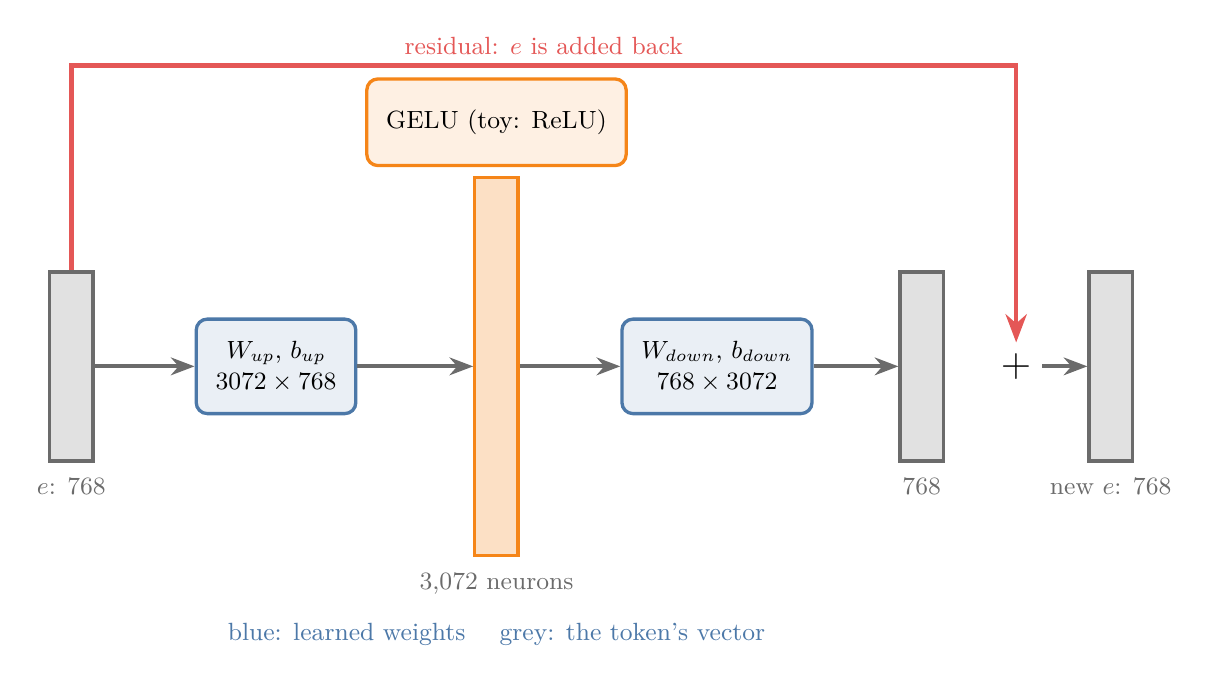
\begin{tikzpicture}[v/.style={draw=cgrey, fill=cgrey!20, minimum width=0.55cm, inner sep=0pt},
  w/.style={box=cblue, minimum height=1.2cm, font=\sffamily\small}]
  \node[v, minimum height=2.4cm] (e) at (0,0) {};
  \node[note, below=2pt of e] {$e$: 768};
  \node[w] (up) at (2.6,0) {$W_{\text{up}}$, $b_{\text{up}}$\\$3072 \times 768$};
  \node[v, minimum height=4.8cm, fill=corange!25, draw=corange] (n) at (5.4,0) {};
  \node[note, below=2pt of n] {3,072 neurons};
  \node[box=corange, font=\sffamily\small] at (5.4,3.1) {GELU (toy: ReLU)};
  \node[w] (down) at (8.2,0) {$W_{\text{down}}$, $b_{\text{down}}$\\$768 \times 3072$};
  \node[v, minimum height=2.4cm] (o) at (10.8,0) {};
  \node[note, below=2pt of o] {768};
  \node[font=\sffamily\Large] (plus) at (12.0,0) {$+$};
  \node[v, minimum height=2.4cm] (e2) at (13.2,0) {};
  \node[note, below=2pt of e2] {new $e$: 768};
  \draw[arrow] (e) -- (up); \draw[arrow] (up) -- (n); \draw[arrow] (n) -- (down); \draw[arrow] (down) -- (o);
  \draw[arrow] (plus) -- (e2);
  \draw[cred, line width=1.6pt, -{Stealth}] (e.north) -- ++(0,2.6) -| node[pos=0.25, above, note, text=cred] {residual: $e$ is added back} (plus.north);
  \node[note, text=cblue] at (5.4,-3.4) {blue: learned weights \quad grey: the token's vector};
\end{tikzpicture}
\end{document}
